\documentclass[a4paper,10pt]{scrartcl}
\usepackage[german,ngerman]{babel}
\usepackage[utf8]{inputenc}
\usepackage[T1]{fontenc}
\usepackage{lmodern}
\usepackage{fullpage}
\usepackage{tikz}
\usepackage{multicol}
\usepackage{wrapfig}
\usepackage{droid}
\usepackage[colorlinks, pdfpagelabels, pdfstartview = FitH, bookmarksopen = true,bookmarksnumbered = true, linkcolor = black, plainpages = false, hypertexnames = false, citecolor = black] {hyperref}

\author{Ein Subset des inf12-Jahrgangs}
\title{Was man über IKON 1 wissen sollte}
\date{Irgendwann zwischen Vorlesungen und Klausur}

\pagestyle{plain}

\renewcommand{\headheight}{12pt}
\renewcommand{\headsep}{12pt}

\setlength{\parindent}{0pt}
\setlength{\parskip}{0.6em}
\linespread{1.2}

\begin{document}
\setcounter{secnumdepth}{0}

\maketitle
\tableofcontents

\newpage
\section{01 - Einleitung}

Der Mensch und der Computer sind gut erforscht, nur die Verbindung dazwischen nicht: ,,missing link''.

Schreiben: Schrift entsteht am Werkzeug. Tippen: Schrift entsteht woanders - man muss ,,blind tippen''.

Maus: Hand-Auge Koordination, Alignment!

\subsection{Computersysteme zur Problemlösung}

Ist die Interaktion zwischen Benutzer und Computer kognitiv und perzeptiv auf den
Benutzer abgestimmt? Versteht der Benutzer, was der Computer tut? Versteht der
Benutzer, was er tun muss?

Das \textbf{Herddesign}-Beispiel zeigt, wie die Anordnung der Knöpfe beim \emph{natural mappings}-Design
an die Fähigkeit/Eigenschaft des Menschen angepasst werden, nämlich die Anordnung
analog von den Schaltern auf die Platten anzuwenden.

Eine \textbf{Uhr} soll einfach/schnell und präzise/korrekt abgelesen werden können.
Vorteil der Analoguhr: kein Zahlenverständnis. Vorteil der Digitaluhr: einfaches
Ablesen. Negativ-Beispiel: Berlinuhr (es muss \emph{gerechnet} werden).

\newpage
\section{02 - Grundlagen der Informationsverarbeitung}

Die \textbf{Informatik} befasst sich mit Informationen. Die
\textbf{Kognitionswissenschaft} beruht auf der Informationsverarbeitung.
\textbf{Kognitive System} (oder ,,Agenten'') sind gemeinsames Forschungsthema.

\textbf{Daten} sind Artefakte, welche Inhalte speichern. \textbf{Eine Information}
lässt sich aus Daten interpretieren, wenn ein Zusammenhang (Vorwissen, Hintergrundwissen,
aktuelle Umgebung) gegeben sind. \textbf{Wissen} ergibt sich aus einer Anhäufung
relevanter Informationen und deren Anwendung.

\begin{tabular}{|p{20em}|p{15em}|}
\hline
Das System muss auf Fähigkeiten des Menschen angepasst sein
& Kenntnisse über Kognition, Perzeption, Motorik\\ \hline

Der Mensch muss verstehen, was das System tut
& Ein- und Ausgabeschnittstellen \\ \hline

Kommunikation zwischen Computer und Mensch muss ,,funktionieren''
& Prozesse der Interaktion\\ \hline
\end{tabular}

Menschen sind nur sehr eingeschränkt in der Lage, kognitive und perzeptive Fähigkeiten
durch Training zu verbessern (Beispiel: Blinde hören nur etwas besser als sehende Menschen).

Eingabeinformationen werden durch eine Operation (möglicherweise komplexe Operation bestehend
aus mehrerenen elementaren Operationen) in Ausgabeinformationen überführt, die wiederum zu
Verhalten/Aktionen führen.

Die interne Struktur ist nicht immer zu beobachten (Black Box), nur das Verhalten. Empirisch
(Experiment und Beobachtung) lässt sich in beschränktem Umfang auf die Operation schließen.

\newpage
\section{03 - Neurowissenschaftliche und Neuroinformatische Grundlagen}

\textbf{Sensor-Neurone} erkennen physikalische/chemische Signale, \textbf{Motor-Neurone}
steuern die Muskelkontraktion, \textbf{Interneurone} übertragen die Signale.

Interneurone haben 2 Funktionen: Integration der Eingangs-Information und Weiterleitung
an andere Neurone.

Hirnregionen haben spezielle Aufgaben, allerdings nicht ausschließlich. Eine Region kann
auch Neuronen enthalten, die andere Aufgaben ausführen, und gewisse Neuronengruppen können
auf ,,fremde'' Aufgaben übernehmen (\emph{Plastizität}). Diese nicht-exklusive Einteilung
heißt \textsc{Large Grain Feature}.

Neuronen empfangen Signale an den \emph{Dendriten}, integrieren diese am \emph{Zellkörper}, leiten
sie über die \emph{Axone} zu den \emph{Terminalen}, wo sie an \emph{Synapsen} an die Dentriten anderer
Neuronen weitergegeben werden. \emph{Exzitatorische} Synapsen erhöhen den Eingabe-Wert,
\emph{inhibitorische} verringern ihn. Wird ein Schwellwert (\emph{threshold}) erreicht, ,,feuert'' das Neuron.

In künstlichen \emph{neuronalen Netzen} wird dies simuliert. Eingabeverbindungen werden
mit den Konnektions-Gewichten multipliziert und zum inneren Produkt addiert (1. Phase). In einer 2. Phase
wird dieser Wert durch eine Funktion abgebildet auf einen Ausgangs-Wert. Diese Funktion
kann unter anderem linear, beschränkt linear, nichtlinear oder treppenförmig (Schwellwert) sein.

Neuronen im Gehirn sind zwar stark vernetzt, jedoch nicht nur regional, sonder weit
verteilt. Das ist wichtig für \emph{Vorwärts- und Rückwärtsprojektion}, um Informationen
aus verschiedenen Arealen zu kombinieren (z.B. Hintergrundwissen und visuelle Information).

\newpage
\section{04 - Wahrnehmung}

\subsection{Visuelle Wahrnehmung}

Palmer's 4-Stufen-Modell: Retinal Image (2D Projektion)
$\rightarrow$ Image (Bildatome, z.B. Kanten)
$\rightarrow$ Surfaces (Zusammengehörende Flächen)
$\rightarrow$ Objects (3D-Objekte, Tiefensinn)
$\rightarrow$ Categories (Einschätzung, Interpretation).

Die \textbf{Retina} ist die Netzhaut, und enthält Stäbchen und Zapfen als Sensorzellen
sowie davor Bipolar-, Amakrin-, Horizontal- und Ganglienzellen zur Verarbeitung
und Sammlung der Informationen und Weiterleitung über den Sehnerv.

Jede Ganglienzelle ist mit mehreren Sensorzellen verknüpft, der Bereich heißt
\textbf{Rezeptives Feld}. Die verschiedenenen rezeptiven Felder überlappen sich, die
Informationen werden also mehrfach verwendet.

Der Bereich mit der höchsten Zapfendichte heißt
\textbf{Fovea}, und hat etwa 0.5mm Durchmesser. In diesem Bereich sind keine anderen
Zellen den Sensorenzellen vorgelagert. Hier hat man optimale Schärfe, aber wegen
der Bauart kann nur ein kleiner Bereich so gestaltet sein. Daher muss man das
Auge bewegen, um die Umwelt wahrzunehmen.

\textbf{Zapfen} sind farbempfindlich (rot/grün/blau), und besonders scharf in der Mitte.
\textbf{Stäbchen} sind sehr lichtempfindlich, funktionieren also nicht bei starker
Helligkeit, dafür ermöglichen sie Nachtsehen. Sie sind mehr in der Peripherie angeordnet
als im Zentrum.

Der Sehwinkel des Menschen beträgt etwa $1^\circ$. Dies entspricht einer Länge von 12pt bei
einem Abstand von 30cm. Die Darstellungsgröße, etwa von Schrift, muss daher auf das
Medium angepasst werden. Je weiter weg von der Fovea, desto größer muss etwas dargestellt
werden, um erkennbar zu sein.

\begin{center}
    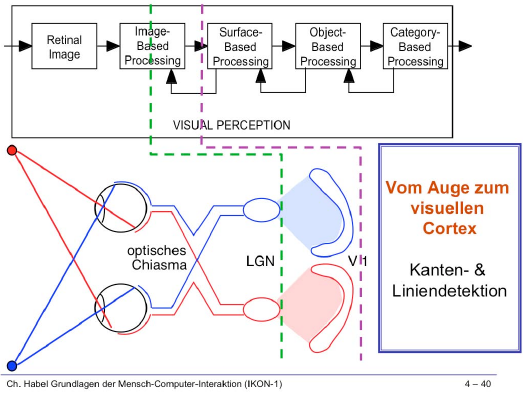
\includegraphics[width=0.7\textwidth]{eye-visual-cortex.png}
\end{center}

Durch verschiedene Verschaltung von rezeptiven Feldern ist es möglich, Kontrast-Kanten
zu erkennen. Ähnlich funktioniert computationelle Kantenerkennen. Der Kantenoperator
bildet die Differenz in der Intensitätsmatrix zweier benachbarter Zellen, entweder
horizontal oder vertikal (horizontaler Kantenoperator heißt, er erkennt horizontale
Kanten, wendet also auf vertikal benachbarte Zellen an). Im neuronalen Netzwerk ist
der Kantenoperator über exzitatorische und inhibitorische Verbindungen aufgebaut (Differenz).

Das Auge kann im \textbf{dreidimensionalen Farbraum} wahrnehmen. Der Farbraum hat dabei
die 3 Dimensionen Helligkeit (\emph{lightness}), Sättigung (\emph{saturation}) und
Farbton (\emph{hue}), wobei die letze Dimension zyklisch ist.

Nach intuitivem Farbempfinden gibt es 3 Paare komplementärer Farben: schwarz -- weiß,
rot -- grün und blau -- gelb.

Die ,,Luminanz'' einer Farbe beinhaltet nicht den Blauwert - daher ist von Details
mit konstanter Luminanz, etwa gelber Schrift auf einem Blau-Weiß-Verlauf, abzusehen
(Luminanz wird für Detailkontrast benötigt). Da außerdem die blauen Zapfen am geringsten
ausgeprägt sind, ist von blauem Text auf dunklem Hintergrund ebenfalls abzuraten.

\subsubsection{Tiefenwahrnehmung}

Wichtig für die Tiefenwahrnehmung sind die Distanz vom Objekt sowie die Ausrichtung
der Oberflächen (Vektor der Oberflächennormalen). Größere Objekte werden als ,,näher
dran'' empfunden. Dies kann zu Illusionen führen. Der Oberflächenvektor wird leicht
über den Lichteinfall und die resultierende Schattierung (\emph{shading}) erkannt.

\subsubsection{Objekterkennung}

Für die Objekterkennung wird das wahrgenommene Bild im Arbeitsgedächtnis mit bekannten
Objekten/Eindrücken aus dem Langzeitgedächtnis kombiniert.

\subsection{Das 2-Stufen-Modell der Wahrnehmung}

Wahrnehmung kann in 2 Stufen unterteilt werden. In der ersten Stufe wird parallel
und ohne Aufmerksamkeit (präattentiv, bottom-up) automatisch und schnell von Neuronenverbunden
verarbeitet. Die Information wird nur sehr kurz gespeichert. Im 2. Schritt wird
bewusst und zielgerichtet weiterverarbeitet, dies dauert länger und kann nicht
parallelisiert ablaufen (top-down).

Menschen können somit die Anzahl von Objekten im Sehfeld auch bei nur kurzer
Betrachtungsdauer (bis 400 ms) erkennen, ohne zählen zu müssen, wenn es sich um eine
kleine Anzahl Objekte handelt (3 - 8). Dieser Effekt heißt \textbf{subitizing}, und
ist im Gegensatz zum Zählen präattentiv. Ähnliche Phänomene sind \textbf{multiple object
tracking} (verfolge sich bewegende Objekte und indentifizieren hinterher die vorher
markierten) und \textbf{change blindness} (Dinge verändern sich, während die Aufmerksamkeit
auf andere Objekte gelenkt wird).

\subsection{Haptische Wahrnehmung}

... basiert auf Drucksensoren unter der Haut sowie kinesthethischen Rezeptoren in Muskeln,
Sehnen und Gelenken. Der haptische Sinn ist direkt, nur Objekte, mit denen Kontakt besteht,
können erfasst werden (Ausnahme: Hitzestrahlung).

Im Gegensatz zur visuellen Wahrnehmung ist die haptische Konturenerkennung von 2D-Objekten
sequentiell.

\newpage
\input{kapitel-05.tex}
\newpage
\section{Glossar}

\begin{description}

\item[Agent] Natürliches oder künstliches System mit gewissen Eigenschaften (Oberbegriff).

\item[Ergonomie] Wissenschaft der Leistungsmöglichkeit und -grenzen von Menschen. Anpassung
    der Arbeitsumgebung an menschliche Fähigkeiten.

\item[Kognition] Prozesse des Denkens (Folgern, Probleme lösen),
    Kommunizierens (Sprache, Gestik, Grafik), Gedächnis

\item[Kognitive Artefakte] Objekte zur Unterstützung der menschlichen Kognition,
    Werkzeuge zur Unterstützung \emph{geistiger Prozesse}.

\item[Large Grain Feature] Nicht-exklusive Einteilung der Gehirnareale nach kognitiver
    Funktion, vgl. \textsc{Phrenologie}.

\item[Motorik] Fähigkeit der Bewegung (Gehen, Greifen)

\item[Perzeption] Wahrnehmung (Sehen, Hören, Tasten, ...)

\item[Phrenologie] Zusammenhang zwischen kognitiver Funktion und Areal des Gehirns.

\end{description}


\end{document}
